\section{Methods} \label{sec:methods}

The goal of this work is to develop empirically-informed best practice recommendations for using hereditary stratigraphy methods to trace ancestry relationships in digital evolution.
This section begins with the conceptual basis of the hereditary stratigraphy approach, covering the checkpoint-based strategy used to measure relatedness.
Guidance developed in this work, in particular, investigates two technical aspects of hereditary stratigraphy annotation:
\begin{enumerate}
\item checkpoint retention policy (steady vs. tilted), and
\item checkpoint storage strategy (column vs. surface).
\end{enumerate}
A subsection is provided detailing each of these algorithmic facets.

Having introduced the algorithmic structure of hereditary stratigraphy, attention turns to experiments conducted to evaluate which algorithmic configurations achieve best reconstruction quality.
To be able to make general recommendations, where necessary tailored to application characteristics, we evaluated reconstruction quality across a variety of use case scenarios.
Discussion covers the model used to generate reference phylogenies and the set of treatments evolutionary scenarios varying in scale and ground-truth phylogenetic richness explored.
Finally, we describe metrics used to measure reconstruction quality, statistical methods, and software used for reconstruction quality experiments.
% We describe the model system used, and the different treatments explored to test the effects of evolutionary conditions and evolutionary scale.

\subsection{Hereditary Stratigraphy}

Hereditary stratigraphy obtains phylogenetic information in manner akin to how molecular phylogenetics approaches infer relatedness from comparisons among the genomes of biological organisms, which relies on the tendency for organisms with close hereditary relatedness to exhibit greater sequence similarity \citep{yang2012molecular}.
However, phylogenetic analyses of sequence similarity under a mutational drift model is a nontrivial statistical problem \citep{neyman1971molecular} that can be computationally demanding \citep{konno2022deep,stamatakis2013novel}, data intensive (upwards of thousands of base pairs per genome) \citep{parks2009increasing,cloutier2019whole,wortley2005much}, and hindered by challenges arising from back mutation, mutational saturation, selection effects, and branch length differentials \citep{brocchieri2001phylogenetic,moreira2000molecular}.
Although genome sites under mutational drift can be used to estimate relatedness among digital organisms \citep{moreno2021case}, a more lightweight and robust approach is desirable.
To meet this need, hereditary stratigraphy systematizes a regimen of structured mutation that enables high-quality inference from small amounts of genetic material \citep{moreno2022hereditary}.
The result is a general-purpose framework for phenotypically-neutral ``annotations'' that can be affixed to digital organisms' genomes, or individual genes, to make their lineages traceable \citep{moreno2022hstrat}.

Hereditary stratigraphy works through a simple checkpointing procedure.
Each generation, annotations are extended by appending a new random ``fingerprint'' value.
These fingerprints, referred to as ``differentiae'' in the context of hereditary stratigraphy, serve to chronicle lineage history.
The first pair of mismatching differentiae between two records definitively indicates a split in ancestry.
Conversely, insofar as two annotations share identical differentiae, they likely share common ancestry.

Because differentiae are randomly generated, it is possible that they collide by chance.
The frequency of such spurious collisions depends on the size of fingerprint values used, e.g., a single bit, a byte, a 32-bit word, etc.
Smaller differentiae reduce annotations' memory footprint, but make overestimation of relatedness more likely.
Annotation memory use can also be reduced by discarding old differentiae as generations elapse.
However, sparse retention reduces the number of reference points where divergence between lineages can be tested for.
These two mechanisms enable tunable trade-offs between annotation size, inference precision, and inference accuracy.
As such, strategies for differentia sizing and differentia retention are tested in reconstruction quality experiments, described below, to synthesize recommendations for best practice.
The following section delves into the primary dimension of retention policy, steady versus tilted distribution, considered in this work.

\subsection{Steady and Tilted Retention Algorithms}

\begin{figure}
  \centering
  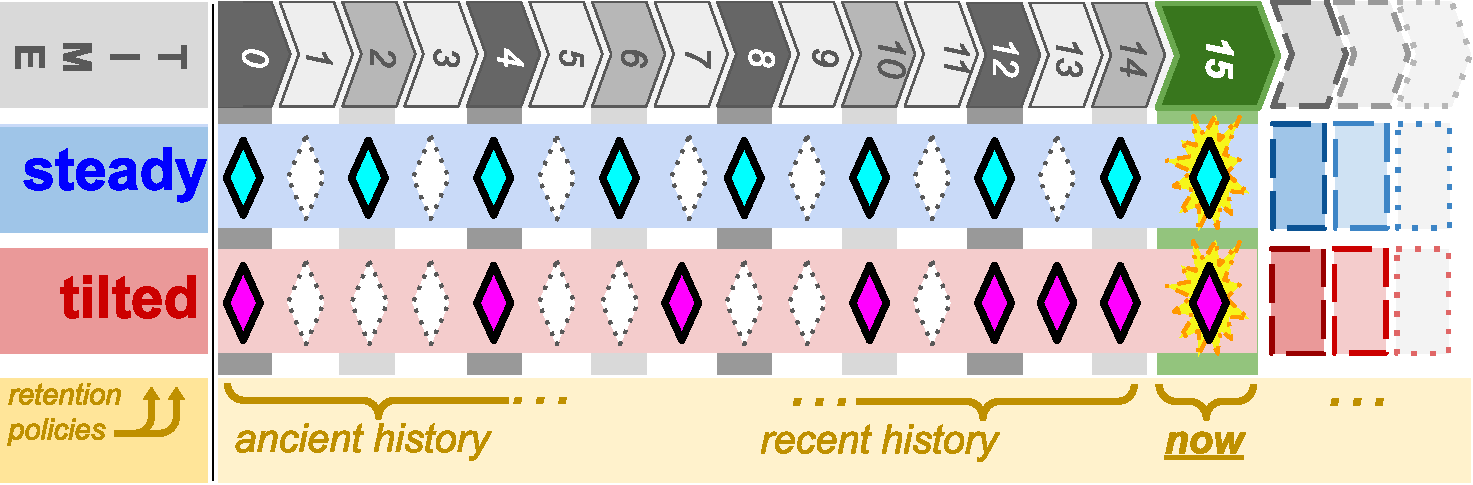
\includegraphics[width=\linewidth]{img/steady-vs-tilted-schematic}
  \caption{%
  \textbf{Steady versus tilted retention policy.}
  Steady policy (top) retains differentia with time points spaced evenly across history.
  Tilted policy (bottom) retains differentia more densely over recent history, giving gap size proportional to time ago.
  Hybrid policy (not shown) allocates half of available space to hold tilted data and half to hold steady.
  }
  \label{fig:steady-vs-tilted-schematic}
\end{figure}


When pruning differentiae, care must be taken to ensure retention of checkpoint generations that maximize coverage across evolutionary history.
In one possible strategy, retained time points would be spread evenly across history.
We term this strategy as ``steady'' \citep{han2005stream,zhao2005generalized}.
Such an approach ensures that last common ancestor (LCA) events can be discerned with consistent precision, no matter when they occured.

Although the steady approach minimizes worst-case imprecision, there is reason to believe it may fail to allocate precision where it is most useful to discern phylogenetic topology.
In most evolutionary scenarios, there is a consistent tendency for phylogenetic events concerning extant taxa to be more tightly packed in the near past \citep{zhaxybayeva2004cladogenesis}.
A strategy accounting for this fact would retain newer time points at higher density than older time points.
We call such an approach, where differentiae are retained in a recency-proportional manner, as ``tilted'' \citep{han2005stream,zhao2005generalized}.
Preliminary experiments have indicated that, at least in some scenarios, annotations using tilted retention can yield higher quality phylogenetic reconstructions than with steady retention \citep{moreno2022hereditary}.
Experiments in this work addresses this question more thoroughly, to assess the relative performance over a variety of evolutionary scenarios, including those expected to maintain greater amounts of ancient history.
In addition, to assess whether benefits of these two approaches can be combined, some experiments consider a third, ``hybrid''' strategy, where half of annotation space is split evenly between steady and tilted strategies.

Figure \ref{fig:steady-vs-tilted-schematic} provides a visual comparison of steady and tilted retention strategies.
The steady history spaces retained differentia at regular intervals, while gap sizes progressively decrease with recency under the tilted policy.
To fully appreciate the mechanics of differentia retention, however, an additional dimension of time must be considered.
Rather than deciding retention just at one particular fixed point in time, these policies must handle continual accrual of new differentia as generations elapse.
At each step, a new differentia is appended, as required, old differentia are discarded.
Throughout, constraints on time point coverage and annotation size must be respected.
Differentia curation for hereditary stratigraphy, indeed, turns out to be an instance of a larger class of ``stream curation'' problems where temporally-representative records must be maintained on a rolling basis.
For elaboration on this point, and more on the implementation and algorithmic properties of retention policies, see \citet{moreno2024algorithms}.

\subsection{Column and Surface-Based Algorithms}

Having just described approaches to deciding which differentiae should be stored, we now pivot to consider approaches to actually organize and store them.
A suitable annotation data structure for differentiae curation should:
\begin{enumerate}
\item support efficient update operations (to append new differentia and discard old differentiae),
\item be readily serialized (to exchange annotated genomes between simulation processes), and
\item minimize representational overhead (to minimize annotation memory footprint and inter-process message size).
\end{enumerate}

The last point, minimizing representational overhead, is particularly critical given in use cases calling for single-bit and single-byte differentiae.
Were 32- or 64-bit pointers or time point values to be required per differentia, bookkeeping overhead would greatly outweigh, and potentially crowd out, actual lineage history information that could be stored.
As such, both approaches considered here --- ``column'' and ``surface''-based storage --- pack differentiae in an array format and rely on positional context to identify them.
Note that for such data to be readily legible, retention policies' curated time points must be directly enumerable \textit{a priori} for any arbitrary generation.

The ``column''' approach arranges differentia in chronological order, with newest differentia stored last.
This approach suits use of a dynamic array data structure (e.g., Python \texttt{list}/C++ \texttt{std::vector}) to store differentiae, as new additions can be accessioned through an append (e.g., ``\texttt{push\_back}'') operation.
Accordingly, arbitrary curated collection growth can be supported.
This allows for retention policies that provide hard guarantees for inference precision.
\footnote{%
Hard fixed or recency-proportional bounds on differentia gap sizes require orders of growth in retention that are linear and logarithmic, respectively \citep{moreno2024algorithms}.
}
One disadvantage to this approach, though, is that discarding old differentia requires a shift-down operation on all subsequent elements.

The ``surface'' approach, in contrast, organizes differentiae directly onto a fixed-length buffer.
Rather than appending as a ``\texttt{push\_back}'' on the array, incoming differentiae are assigned an arbitrary buffer position and directly written there.
One advantage of this approach is that separate garbage collection operations streamline away: new data simply overwrites that to be discarded.
Another advantage is full use of available space: after the surface buffer is filled, it is guaranteed that stored differentiae fully utilize available capacity.
Owing to discrepancy between projected upper bounds on retained size and actual usage, this is not the case for size-capped tilted retention using columns.
However, to the surface's disadvantage, dropping a level of abstraction to operate over buffer sites rather than differentia time points results in less fine-grained control over retention and, particularly in the case of size-capped steady retention, a somewhat looser adherence to idealized retention patterns.
Additionally, by design, orders of growth beyond the surface's fixed buffer size (e.g., logarithmic, linear) are not supported.
For a more detailed description of motivation and implementation of surface-based algorithms, see \citep{moreno2024trackable}.

In sum, the question of column- versus surface-based algorithms can be characterized as a trade-off between efficiency and exactitude.
Indeed, we have found surface-based algorithms to provide order-of-magnitude speedups, as well as good compatibility with low-level, resource-constrained programming environments (notably, the Cerebras Wafer-Scale Engine hardware accelerator) \citep{moreno2024TODO}.
To assess how, if at all, this trade-off impacts reconstruction quality, we include trials using both approaches in empirical annotate-and-reconstruct experiments, described below.
Note that, in these experiments, we consider only fixed-size annotations.
However, we anticipate nearly all hereditary stratigraphy use cases will apply fixed-size annotation, due to benefits from avoiding dynamic memory allocation and variable-length inter-process messaging at runtime.

\subsection{Model System}  %TODO this section needs to be paraphrased

This section describes the used to generate reference phylogenies from
Our goal in performing tests of reconstruction quality is to systematically alter the tree structure, with strong manipulations.
We focused on manipulating phylogenetic richness, doing this by increasing spatial and ecological structure, which are known to increase richness \citep{moreno2024ecology,gomez2019understanding,valiente2007facilitation}.
Tree imbalance, this is like increasing the taxa count on part of the tree.
We manipulate taxa count as its own experimental treatment.
Experiments testing the relationships between evolutionary dynamics, reconstruction error, and phylogenetic structure required a model system amenable to direct, interpretable tuning of ecology, spatial structure, and selection pressure.
Finally, a parsimonious and generic model system was desired so that findings would better generalize across digital evolution systems.
The core of this work relies on a simple agent-based model devised to fulfill these objectives.

Genomes in our model comprised a single floating-point value, with higher magnitude corresponding to higher fitness.
Extensions of hereditary stratigraphy to sexual lineages are possible \citep{moreno2024methods}.
However, lineages used in this work were asexual in nature.
Selection was performed using tournament selection with synchronous generations.
Mutation was applied after selection, with a value drawn from a unit Gaussian distribution added to all genomes.
Evolutionary runs lasted 100,000 generations.
We also sought to understand the relationship between population scale and reconstruction quality.
Population sizes of 4,096 ($2^{12}$) and 65,536 ($2^{16}$) were used for all experiments.
We anticipate that in the majority of use cases, trees will be downsampled for tractability of phylogenetic analysis and reconstruction.
As such, we were also interested in how the downsampling level related to reconstruction quality.
We tested two downsampling levels: 500 taxa and 8,000 taxa (on the largest population size).

Treatments incorporating spatial structure used a simple island model.
In spatially structured treatments, individuals were evenly divided among islands and only competed in selection tournaments against sympatric population members.
Islands were arranged in a one-dimensional closed ring and 1\% of population members migrated to a neighboring island each generation.

Treatments incorporating ecology used a simple niche model.
Population slots were split evenly between niches.
Organisms were arbitrarily assigned to a niche at simulation startup and were only allowed to occupy population slots assigned to that niche.
Therefore, individuals exclusively participated in selection tournaments with members of their own niche.
In treatments also incorporating spatial structure, an even allotment of population slots was provided for every niche on every island.
Every generation, individuals swapped niches with probability $3.0517578125 \times 10^{-8}$ (chosen so one niche swap would be expected every 500 generations at the larger population size and 4,000 generations at the smaller). 

\subsection{Experimental Treatments}

For our main experiments, we defined the following ``regimes'' of evolutionary conditions:
\begin{itemize}
  \item \textit{plain}: tournament size 2 with no niching and no islands,
  \item \textit{mild structure}: tournament size 2 with 2 niches and 4 islands,
  \item \textit{rich structure}: tournament size 2 with 8 niches and 64 islands,
  \item \textit{drift}: tournament size 1 with no niching and no islands,
\end{itemize}

% for num_generations in 10000 100000; do
% for scope in "export population_size=4096 downsample=500" "export population_size=65536 downsample=500" "export population_size=65536 downsample=8000"; do
% for instrumentation in "export annotation_size_bits=32 differentia_width_bits=1" "export annotation_size_bits=64 differentia_width_bits=1" "export annotation_size_bits=256 differentia_width_bits=1" "export annotation_size_bits=256 differentia_width_bits=8"; do
% for stratum_retention_algo in "surf-steady" "surf-tilted" "surf-hybrid" "col-steady" "col-tilted"; do

% for condition in "export num_islands=1 num_niches=1 tournament_size=2" "export num_islands=1 num_niches=1 tournament_size=1" "export num_islands=4 num_niches=2 tournament_size=2" "export num_islands=64 num_niches=8 tournament_size=2"; do

Across all experiments, each treatment comprised 20 replicates.

This model system has been established to generate reference phylogenies in existing work \citep{moreno2023toward,moreno2024ecology}.

We test five capacities and configurations of fingerprint retention.
\begin{itemize}
  \item 32-bit array,
  \item 64-bit array,
  \item 256-bit array, and
  \item 32-byte (256-bit size) array.
\end{itemize}

For the column-based algorithms, this was a size cap.
For the surfface-based algorithms, this was a buffer size.

This work uses 1 byte differentiae, which collide with probability $1/256$, and 1 bit fingerprints, which collide with probability $1/2$.
Greater space efficiency could be achieved using 1 bit fingerprints.
However, this would require careful accounting for ubiquitous generation of identical fingerprints by chance and is left to future work.

As a final point of clarification, r
Orthogonal to the question of steady- and tilted-policy surface-based hereditary stratigraphy algorithms have been developed and thoroughly tested, though they have not yet been formalized.

\subsection{Agglomerative Reconstruction}

In order to , it is necessary to actually build the trees.
Implemented in the \texttt{build_tree} method in the \textit{hstrat} Python package \citep{moreno2022hstrat}.
We devised an agglomerative tree building algorithm that works by successively adding leaf organism annotations and percolating them down from the tree root along the tree path of internal nodes consistent with their fingerprint sequence, then affixing them where common ancestry ends \citep{moreno2024analysis}.
% @MAM did the test under drift conditions
Building took less than a second for the 500 leaf tree with the 256-bit annotation.
In optimized mode, the 256-bit annotation takes about 5 seconds to build the 8,000 leaf tree.
We added a postprocessing step that takes 20 seconds.
Part of the reason this is so fast is that we have synchronous generations.
Asynchronous generations can run slower, owing to complications around missing differentia.
In other work, we found that the current pure Python implementation built trees of 10,000 nodes in around an hour, at a rate slightly faster than 2 nodes per second under optimizations \citep{moreno2024trackable}.
Optimized implementation in a compiled language is on the project roadmap, which we hope will speed this process up.
We are also interested in exploring ways reconstruction implementation could leverage parallelization, owing to potential to rapdily sort taxa between the first n subtrees according to their initial differentia.

To generate reconstructed trees in experiments, we simulated the inheritance of hereditary stratigraphic annotations along a reference phylogeny to yield the set of annotations that would be attached to extant population members at the end of a run, then used our agglomerative tree building technique.
Thus, each reconstruction replicate has a directly-corresponding reference tree from a perfect-tree treatment replicate.
Figure \ref{fig:plain-perfect-and-reconstruction-phylogenies} shows a reference tree and corresponding reconstructions performed using 32-bit, 64-bit, 256-bit, and 32-byte (sized 256 bits) differentia arrays hereditary stratigraph annotations.


\subsection{Reconstruction Quality Measures}

There are two failure modes where reconstruction can fail.
property of hereditary stratigraphy
Even in single-bit differentia, more than two records can be completely identical by chance.
These will be reconstructed as a polytomy at the leaves.
In the first, the reconstruction gives
We used two measures of reconstruction quality.

The first is accuracy.
We used triplet distance as an accuracy measure.
This measure samples random sets of three leaf nodes and checks whether their topology matches between two trees.
To assess the efficacy of the new agglomerative tree-building approach, we calculated all reconstructed trees' triplet distance to their respective reference.
Triplet distance ranges from 0 (between identical trees) to 0.5 (between random trees) to a hypothetical maximum of 1.0, providing in this case a measure of reconstruction error.

To complement accuracy, we also considered a precision measure, the fraction of nodes recovered.
This helps to zero in on the the error introduced due to imprecision.

\subsection{Effect-size Analysis}

To best inform practicioners, we sought to assess the consistency with which one type of instrumentation outperformed another across replicates.
Cliff's delta provides useful nonparametric means for such effect size analysis.
This statistic reports the proportion of distributional non-overlap between two distributions, ranging from -1/1 if two distributions share no overlap to 0 if they overlap entirely \citep{meissel2024using,cliff1993dominance}.
When reporting effect size, we use conventional thresholds of 0.147, 0.33, and 0.474 to distinguish between negligible, small, medium, and large effect sizes \citep{hess2004robust}.

Note that the Cliff's delta statistic tops/bottoms out entirely once two distributions become completely separable.
Although this property suits most analyses performed, it is occasionally useful to distinguish the extent of divergence between phylometric distributions past the point of complete separability.
For these purposes, we perform a simple procedure to normalize phylometrics relative baseline conditions by subtracting out the baseline mean and dividing by the baseline standard deviation.

We typically pair effect-size analysis with Mann-Whitney U testing in order to assess the extent to which differences between phylometric readings under different conditions are, or are not, evidenced by available data \citep{mann1947on}.
As a final detail, note that we typically report negated Cliff's delta values where necessary to ensure positive values correspond to larger phylometric values and vice versa.

\subsection{Software and Data Availability}

Software, configuration files, and executable notebooks for this work are available at \url{https://doi.org/10.5281/zenodo.11178607}.
Data and supplemental materials are available via the Open Science Framework \url{https://osf.io/n4b2g/} \citep{foster2017open}.

All hereditary stratigraph annotation, reference phylogeny generation, and phylogenetic reconstruction tools used in this work are published in the \textit{hstrat} Python package \citep{moreno2022hstrat}.
This project can be visited at \url{https://github.com/mmore500/hstrat}.
For interchangeability/consistency, and owing to the recent creation of the surface-based herediitary stratigraphy, and the underlying downstream curation algorithms behind it, all experiments used the \texttt{HereditaryStratigraphicColumn} impelementation from \texttt{hsttrat}.
We used a shim to convert the retention patterns that would occur under surface site selection algorithms to column retention policies.
The site selection algorithms and shim used are provided here \citep{moreno2024hsurf}.
In the medium-term future, we anticipating publishing the surface as a first-class data structure within \texttt{hstrat} and we plan to release the downstream stream curation site selection algorithms in a standalone Python library.

This project uses data formats and tools associated with the ALife Data Standards project \citep{lalejini2019data} and benefited from many pieces of open-source scientific software \citep{ofria2020empirical,sand2014tqdist,2020SciPy-NMeth,harris2020array,reback2020pandas,mckinney-proc-scipy-2010,sukumaran2010dendropy,cock2009biopython,dolson2024phylotrackpy,torchiano2016effsize,waskom2021seaborn,hunter2007matplotlib,moreno2024apc,moreno2024qspool,moreno2023teeplot,hagen2021gen3sis,ofria2004avida,torchiano2016effsize}. % TODO check this